\documentclass[paper=a4, fontsize=11pt]{scrartcl}
\usepackage{amsmath,amsfonts,amsthm}
\usepackage{sectsty}
\usepackage{fourier} % Use the Adobe Utopia font for the document - comment this line to return to the LaTeX default
\usepackage[english]{babel}
\allsectionsfont{ \normalfont\scshape}
\usepackage{fancyhdr}
\usepackage{float}
\usepackage{graphicx}
\usepackage{listings}
\pagestyle{fancyplain}

\fancyhead{} % No page header - if you want one, create it in the same way as the footers below
\fancyfoot[L]{} % Empty left footer
\fancyfoot[C]{} % Empty center footer
\fancyfoot[R]{\thepage} % Page numbering for right footer
\renewcommand{\headrulewidth}{0pt} % Remove header underlines
\renewcommand{\footrulewidth}{0pt} % Remove footer underlines
\renewcommand\floatpagefraction{.9}
\setlength{\headheight}{13.6pt} % Customize the height of the header
\numberwithin{equation}{section} % Number equations within sections (i.e. 1.1, 1.2, 2.1, 2.2 instead of 1, 2, 3, 4)
\numberwithin{figure}{section} % Number figures within sections (i.e. 1.1, 1.2, 2.1, 2.2 instead of 1, 2, 3, 4)
\numberwithin{table}{section} % Number tables within sections (i.e. 1.1, 1.2, 2.1, 2.2 instead of 1, 2, 3, 4)
\setlength\parindent{0pt} % Removes all indentation from paragraphs - comment this line for an assignment with lots of text
\renewcommand{\thesubsection}{\thesection\alph{subsection}}


\setlength\floatsep{1.25\baselineskip plus 2pt minus 2pt}
\setlength\textfloatsep{1.25\baselineskip plus 2pt minus 2pt}



%----------------------------------------------------------------------------------------
%	TITLE SECTION
%----------------------------------------------------------------------------------------

\newcommand{\horrule}[1]{\rule{\linewidth}{#1}} % Create horizontal rule command with 1 argument of height
\title{	
\normalfont \normalsize 
\textsc{Yale-NUS College} \\ [20pt]
\textsc{YID3202C : Data Analysis in Environmental Studies } \\ [25pt] % Your university, school and/or department name(s)
\horrule{0.5pt} \\[0.4cm] % Thin top horizontal rule
\huge Problem Set One \\ % The assignment title
\horrule{2pt} \\[0.5cm] % Thick bottom horizontal rule
}

\author{Jake Goh Si Yuan} % Your name

\date{\normalsize October 16, 2016} % Today's date or a custom date


\begin{document}

\maketitle % Print the title
\section{Fitting Trends Over the Entire Data Series}
\subsection{}
The average increase of $CO_2$ concentration per year from the linear regression model of $CO_2$ concentration with time(with 1958 as origin) is 1.520, and the average increase per decade is 15.20.

\subsection{}
Taking the time data, with origin 0 set as year 1958 and with year 2016 represented as 58, we will arrive at a nominal start-point of 307ppm and endpoint of 395.16ppm\\

The start-point of the data is 315.71ppm or 8.71ppm higher than trend-predicted, and the end-point is 402.25ppm or 7.19ppm higher.
\subsection{}

The standard deviation of the data-misfit residual, or the residual standard error, is 3.871 on 700 degrees of freedom. The F variance ratio, or statistic, is 30880.
\pagebreak
\subsection{}
\begin{figure}[htp]
	\centering
	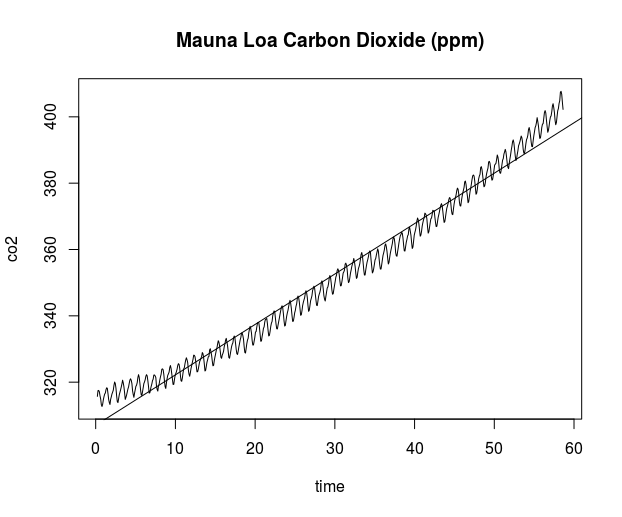
\includegraphics[width=0.7\textwidth, clip]{q1aTime.png} 
	\caption{Regression of time(with 1958 as origin) and Mauna Loa Carbon Dioxide Data}
\end{figure}

The data does not seem to follow strictly to a straight line, in fact, it appears to be have an exponential trend with a small enough exponent that it takes on pseudo-linear characteristics.\\

Also, the linear prediction fails to take into account the saw-tooth motion that the data is taking, or the trend within the trend.


















































\end{document}